\documentclass[11pt]{article}
\usepackage[utf8]{inputenc}
\usepackage{amsmath,amssymb,hyperref,array,xcolor,multicol,verbatim,mathpazo}
\usepackage[normalem]{ulem}
\usepackage[pdftex]{graphicx}
\usepackage{fullpage}
\usepackage{import}
\usepackage{adjustbox}
\usepackage{booktabs}
\usepackage{bbm}
\usepackage[font=footnotesize,labelfont=bf]{caption}
%\captionsetup{justification=raggedright,singlelinecheck=false}


\usepackage[backend=biber,style=authoryear,
sorting=ynt,citestyle=authoryear]{biblatex}
\addbibresource{papercitations.bib}
\usepackage{setspace}
%\singlespacing
\doublespacing
\addtolength{\skip\footins}{2pc plus 5pt}

\title{Labor Markets and Technological Change: Evidence from Electronic Health Records}
\author{Hanna Glenn}
%\date{\today}

\DeclareLabeldate[online]{%
  \field{date}
  \field{year}
  \field{eventdate}
  \field{origdate}
  \field{urldate}
}

\begin{document}

\maketitle



\vspace{1.5cm}

The interaction between technological innovation and labor markets has a direct impact across industries; job characteristics such as displacement, creation, and satisfaction are all prevalent for many workers (\cite{autor2003skill}, \cite{fallick1996review}, \cite{akerlof1988job}). Labor market changes for one job type may have rippling effects on populations serviced by that industry. For example, physician labor markets directly affect patient accessibility and quality of care received. Physician burnout is correlated with lower patient satisfaction (\cite{shanafelt2002burnout}), physician shortages are linked to higher mortality rates (\cite{gong2019higher}), and administrative regulations on physicians such as standardized checklists may be associated with lower mortality in surgical settings (\cite{treadwell2014surgical}). Thus, a shock to physician labor markets have potential implications for healthcare. I investigate physician labor market changes as a result of a major technology shift in the U.S. healthcare system, the implementation of electronic health records, which have been emphasized as a cause of burnout and may induce changes to physician labor market decisions.

Electronic Health Records (EHRs) are computerized medical records which include detailed accounts and notes of medical history, stored in advanced systems with additional capabilities such as providing suggestions for care. EHRs have have become increasingly relevant in the U.S. since 2008, in part after former President Obama stated in 2009, “To improve the quality of our health care while lowering its cost, we will make the immediate investments necessary to ensure that, within five years, all of America’s medical records are computerized.” (\cite{presquote}). The movement towards digitization in health care was expected to have immediate and substantial impacts on efficiency. A 2005 study estimated hundreds of billions of dollars saved if health information technology were to be fully implemented (\cite{hillestad2005}). Such expectations led the U.S. government to incentivize the use of EHRs in hospitals with the the Health Information Technology for Economic and Clinical Health (HITECH) Act in 2009 (\cite{hitech})\footnote{This legislation subsidized hospitals which used EHRs “meaningfully”According to Quatris Healthco, meaningful use standards proceeded in three stages over time. In Stage 1 (2010), MU focused on data capturing and sharing. In Stage 2, which began in late 2012, MU extended to using EHRs for patient incorporation and using the technology as a helper in care. Stage 3 went from 2014-2016 and focused on making data accessible across hospitals (\cite{meanuse})}. The percentage of hospitals with the capability of using a basic EHR system went from 9 percent in 2008 to 84 percent in 2015 (\cite{stats}), revealing the nationwide movement towards digitization.

Physicians, as primary users of this technology, play a meaningful role in whether potential benefits of EHRs are realized. With the rapid implementation of a complex technology, the practical tasks that take place in a physician's daily life changed just as rapidly. In interviews, physicians reported that when using EHRs they are less satisfied with their job and have higher stress levels. Senior physicians in particular were found to “loathe the cumbersome, time-consuming data entry that comes with using EHRs.” (\cite{CollierBurnout}). The frustration of using a new technology raises the cost of working in specific hospitals, which may lead physicians on the margin to make changes in labor market choices such as exiting the labor market altogether or shifting towards other work settings. However, the extent to which this frustration actually imposes a meaningful cost is unknown, making physician response an empirical question. Treating EHR implementation in hospitals as exogenous to an individual physician, I use difference in difference with heterogeneous treatment timing to understand the effect of EHR implementation in hospitals on physician labor market outcomes: retirement, choice of work setting, patients seen, and billing activity.

Using CMS Shared Patient data and Medicare Data on Provider Practice and Specialty (MD-PPAS), I construct a physician-level panel from 2009-2017 consisting of hospitalists and other general practice physicians connected to hospitals. The data captures whether a physician in exposed to EHRs in various hospitals, several labor market outcomes, and demographic information such as zip code, age, and gender. I analyze the impact of EHR exposure on the following physician decisions: (1) retirement, (2) where to physically work (changing hospitals or moving to office based settings), (3) patients seen, and (4) billing activity. Common to each specification is the use of a binary treatment variable capturing a physician's EHR exposure in hospitals. In the main analysis, a physician is considered to be exposed to an EHR if they are working in any hospital that implements an EHR. A key assumption that underlies the main analysis is that exposure is exogenous to individual physicians. That is, the physician does not choose their own EHR exposure. While this assumption is reasonable in many settings, there may be instances where a physician is involved in hospital decision making. For this reason, I include a second definition of EHR exposure that only considers exposure in hospitals where vertical integration between physician and hospital is low, as this indicates a much lower probability that EHR implementation is endogenous. 

I do not observe granular details of what physicians do when they drop out of clinical settings, so I define retirement vaguely as the decision to cease clinical work altogether. Contrary to previous research stating that physicians do not retire based on work environment (\cite{Bahrami2002}), I find that EHR implementation led to a .005 ppt increase (25\% increase relative to the mean percentage) in the likelihood of a senior physician retiring in the year after implementation. Younger physicians were .002 ppts more likely to retire in the second year after exposure, possibly pointing to career switching. Whether physicians are young or old, these results suggest that access to care issues may have been exemplified as EHRs were implemented, and there was a surge of experienced physicians who left the labor force and were no longer available to influence younger physicians learning under them.

Most physicians did not choose to forego clinical work altogether. However, changing physical place of work might be an option if a physician is not satisfied with their current experience at a given hospital, whether it is because of burnout, loss of autonomy, or other factors. I investigate whether physicians switch from primarily hospital based work to office based settings, or more generally switch primary zip codes. I limit the sample to any physicians who did not retire and use the same event study framework to estimate the effect of EHR exposure on switching work settings. I find that younger physicians are .015 ppts more likely to work in an office in the year of exposure to an EHR, but that exposure does not change the average fraction of patients seen in office settings for either age group. Further, when considering a more general outcome of whether a physician switches zip codes, I observe similar trends with even larger magnitudes. This implies that the technology imposed a large enough costs to induce switching and that physicians may be avoiding regulation that imposes loss of autonomy.

Finally, I investigate the effect of the technology implementation on work activity, measured by the number of patients seen, and overall billing activity by the physician. The subtle difference between the two measures represents an important nuance, that an increase in billing activity in itself could actually signify an increase in wastefulness as opposed to productivity if physicians are simply recording more in the EHR system. I find that both the total number of patients and billing activity increases in younger physicians in the first 2-3 years after exposure to an EHR. The ratio of billing activity to patient count increases less than the sample average, suggesting that billing activity did not dis-proportionally increase. 


There is a robust group of empirical papers that examine the effects of EHRs on patient outcomes and hospital costs prior to the HITECH Act taking effect. Despite a large number of case studies that find generally positive effects (improved patient outcomes and decreased costs) (surveyed in \cite{Buntin2011TheResults}), more recent empirical work has found a mixture of results: that the median patient experiences no change due to EHRs (\cite{Agha2014TheCare}, \cite{McCullough2016HealthCoordination}, \cite{Meyerhoefer}) while newborns and severe patients experience improvement in health outcomes (\cite{Miller2009}, \cite{Freedman2015}, \cite{McCullough2016HealthCoordination}), and that hospital costs only decrease 6 years after implementation, if at all (\cite{Agha2014TheCare}, \cite{dranove2014trillion}). More relevant to EHR effects on physicians, a number of studies consider the effect of EHRs on productivity in specific settings. One study finds that nursing home productivity increases after adopting health IT (\cite{Hitt2016}), but another finds that physician productivity decreases by 11 percent due to EMRs being adopted in primary-care sites (\cite{Meyerhoefer}). 

I expand and improve upon this literature, first by considering a different mechanism by which EHRs could indirectly affect patients through physicians' response to them. This is the first study to my knowledge that connects EHR implementation to various physician labor market decisions. Further, I improve on the literature by considering the primary time period in which EHRs were rapidly implemented. This provides sufficient variation in the timing of EHR implementation and ensures the EHRs are advanced enough to be considered "meaningful" by the government's standards, and are likely affecting physicians' daily life. Similarly to past studies, I consider EHR implementation as a treatment variable in a difference-in-difference framework, but I improve on this by estimating average group time treatment effects for multiple years after implementation, which avoids common problems that arise in a typical two way fixed effects setup.  




\section{Institution}

EHRs have been an important feature of healthcare since the 1980s and 1990s. Early in its existence, the technology was mainly produced and used by academic medical centers whose primary goal was to create efficiency in billing and/or scheduling. Prior to computerization, physicians were not able to interface directly with EHRs, and thus were not drastically affected by their implementation. The cost of utilizing an EHR was large and increasing in the amount of capabilities of the system, which led to the widespread view that EHRs were strictly complements to paper records, not a feasible substitute. As computers were made more portable, the usability of EHRs increased, creating what is known as the "physician workspace": a computer station for a physician to interface directly with an EHR to record patient updates. Despite usability, physicians kept the view that EHRs were purely complementary to paper due to burdensome data entry. Automation in data entry was non-existent, making it extremely time consuming for the user. Even when automation was developed for particular machines that performed monitoring, the hospital still held responsibility for the accuracy of information and therefore required physicians to manually check each data entry. 

The HITECH Act was passed in 2009, setting aside government funds to subsidize hospitals who used EHRs according to certain guidelines. The guidelines include having at least 80\% of patients in the system, regularly recording answers to specific questions, and protecting the security of the system to ensure privacy. Immediately, EHR companies took advantage of the legislation and began marketing campaigns centered around their system being eligible to earn the hospital subsidies. Hospitals began receiving payments for the first stage of meaningful use in 2011. This resulted in a 75 percentage point increase in the number of hospitals with EHRs from 2009 to 2015 (\cite{stats}). Figure \ref{fig:meanuse} shows a comparison of U.S. hospitals who have received stage 1 of the meaningful use subsidy in 2011 vs. 2013. 


While EHRs were widely utilized in hospitals by 2015, physicians still continue to report frustration. For every patient seen, a primary care physician spends an average of 16 minutes actively using an EHR, an amount of time that often exceeds face to face time with the patient (\cite{overhage2020physician}). The tasks that may take place during this time include viewing or inputting patient information, ordering services such as tests or prescriptions, navigating the system, or communication. Appendix () includes a computer screen image of what a physician typically sees when looking at an EHR. 

\section{Data}

Using various linked datasets, I construct a physician-level panel spanning from 2009-2017 which measures physicians' exposure to EHRs over time and other relevant characteristics. The different data sets used to construct the panel are described below.

\subsection{MD-PPAS}

Medicare Data on Provider Practice and Specialty is a database of physicians which details claim counts and specialty from 2009-2017. The relevant information included is physician NPI, primary and secondary specialties, both patient and total billing counts in up to 12 different zip codes, and fraction of patients in different settings such as office, inpatient or emergency room. I first limit the sample of physicians based on specialty type. Primary care physicians are exposed to the administrative burden of EHRs in hospitals more-so than specialists. Thus, I only include physicians whose primary specialty is reported as hospitalist, internal medicine, pediatrics, general practice or family practice in at least one year (excluding physicians who have specialist listed in all years but one). Since the focus of the analysis is physicians working in hospitals, I also drop physicians with less than 20\% of patients in a hospital setting in all years, who likely do not have strong ties to the hospitals they have limited work in.

This data includes individual labor market information on physicians which I use to construct the dependent variables for my analysis. Generally, these include the decision to retire (leave clinical work), the decision to switch to a different work setting, number of patients seen and overall billing activity. These outcome variables and their construction are described in detail below.


\subsection{Shared Patient}

CMS Shared Patient data records annual information from 2009 to 2015 on the number of patients who bill two entities under Medicaid in the same day. For example, if a Medicaid patient is referred to a specialist by a primary care physician and the specialist is seen by the patient in the same day, then those two physicians have that shared patient in common. I utilize this data to explore physicians' EHR exposure based on the hospitals they share sufficient patients with. This measure of exposure defines various treatment variables for my analysis. I limit the entities by NPI tax-code to only include shared patients for physician-hospital pairs, where the physicians in these pairs match the physicians from MD-PPAS. I care specifically about primary care physicians who have a close working relationship with hospitals, who do rounds within at least one hospital. The types of physicians are already limited to primary care, but there still may be some office-based primary care physicians in the shared patient data. Therefore, I limit the sample of pairs based on a threshold of same day patients which depends on the number of years the physician appears in the data. Specifically, a physician-hospital pair is dropped if their total number of same day billings with the hospital is less than 30 times the number of years the pair appears in the data. This is because it is important to avoid dropping physicians who leave the data for many years, as this may indicate retirement and skew the results of my analysis.

Using hospital NPI, I link the pairs to the American Hospital Association survey, which contains information on hospital-level EHR use and other characteristics. I record the first year a physician is exposed to an EHR based on implementation in the hospitals they share patients with. I create two measures of EHR exposure. The first is exposure to any EHR in any hospital, which attempts to capture the effect of first-time EHR use on physician labor markets. One concern with this approach is that a typical physician may be involved in the decision to implement an EHR and thus the treatment would be endogenous. While I cannot perfectly address this concern, I define an alternative treatment variable which theoretically will have less likelihood of this endogeneity problem. That is exposure to EHR at a "low integration" hospital (a hospital where physicians have a low measure of vertical integration with the hospital (\cite{madison2004hospital})). In low integrated settings, physicians do not have ownership or much control in the hospital setting. Results for this alternative defintion of exposure are presented in Appendix (). I then aggregate this data to the physician level. Since the Shared Patient data does not extend to 2017 as the MD-PPAS data does, in the analysis I drop physicians who are not treated by 2015 as I do not observe whether they become treated in 2016 or 2017. That is, the data contains no units which are "never-treated".

Finally, I include a physician's graduation year from Physician Compare. I limit to physicians who graduated before 2005, as anyone who graduated medical school after that will be finishing residency during the span of the data and will exhibit labor market changing behavior which could be correlated to EHR exposure purely because of switching work settings during a time of rapid EHR implementation.

\subsection{Outcome Variables}

The first dependent variable I consider is the decision for a physician to retire, or more broadly to stop practicing in a clinical setting altogether. Retirement is constructed as follows: 
$$\text{retire}_{it}=\mathbbm{1}\{FC_{it}=0 \text{ and retire}_{i,t-1}=0\}, $$
where $FC_{it}=\sum\limits_{j=t+1}^T\text{(claim count)}_{ij}$ is all future claims for physician $i$ in year $t$. In words, retire is equal to one in the first year that a physician has no claim counts at any point in the future. I impose that no retirement happens in 2016 since dropping out of the data for one year does not definitively show retirement. Alternatively, I could also define retirement using future number of patients. I use claim count for a more conservative measure of retirement, but using patient count yields identical results.

Next, I consider a physician switching place of work, such as switching to an office based setting or even selecting into different hospitals where preferences may be more aligned. I measure this in the data in three ways. I consider the fraction of patients a physician sees in an office based setting, which is directly available in the data. Further, I use this variable to construct an indicator variable equal to one if a physician sees a positive fraction of patients in an office based setting. There is less variation in this data but allows insight to a different type of decision making where physicians may enter or leave office based setting based on EHR exposure. Lastly, I utilize the zip code information to define an indicator variable equal to one only if the physician's list of zip codes changes from one year to the next. While these variables do not give direct insight into whether physicians specifically move from one hospital to another, they do allow for exploration of whether settings are changing as a result of EHRs in general.

Finally, I consider outcome variables which explore productivity and billing activity once EHRs are implemented in hospitals. Productivity is measured in the number of patients a physician sees in a give year, where the billing activity is the total claim count for the physician. I distinguish between the two because it could be thd case that productivity does not actually increase, but EHRs could encourage excessive billing of things that would not have been billed for otherwise. 

\subsection{Summary Statistics}

Summary statistics for the entire sample are shown in Table \ref{tab:sumstats1}. Only 2\% of physicians retire over the course of the sample, which equates to approximately 750 physicians in the sample who retire at some point. A little over half of the sample works in an office in some capacity, with about a third of the number of patients being seen in an office setting. By construction, all physicians are exposed to an EHR at some point in the sample, so the variation in treatment variables comes from the timing of being exposed. Physicians are typically exposed in any capacity about one fourth of the way through the sample and in low-integrated hospitals about halfway through the sample. The average physician is 48 years old, works with 1.5 hospitals and 1.3 systems. 


I also include a table of means comparing physicians younger than 60, older than 60, and physicians who ever retire (who can fall in either age category) in Table \ref{tab:splitstats}. Senior physicians see more patients and work in more hospitals on average than younger physicians. These older physicians also see a larger fraction of patients in an office setting and are more likely to work in an office in general. Finally, physicians in the higher age bracket are less likely to switch zip codes. The age groups are exposed to EHRs in similar ways, but younger physicians are exposed to EHRs in low integrated setting slightly later. Retirement occurs just as often in the different age groups, indicating the possibility of physicians leaving a clinical setting for an administrative or other position.


In Figure \ref{fig:treatmentgraph}, I present a graph of the variation in treatment variables over time.. In 2009, 32\% of the sample of physicians were exposed to an EHR. That is, three quarters of the sample had no affiliation with EHRs at the beginning of the sample period. Since I drop any physicians who do not have exposure to an EHR by 2015, 100\% of the sample is exposed from 2015-2017. Exposure to EHRs only in low integrated hospitals follows a similar trend with lower exposure rates. When I utilize this treatment variable, I drop all physicians who are not exposed in a low-integration setting by 2015, so the sample of physicians changes according to this limitation. The black line represents the average fraction of a physician's hospitals which are utilizing EHRs over time. Not only are physicians gradually becoming exposed to EHRs, but their exposure is actually increasing over time.


\section{Empirical Strategy}

In this setting, treatment effects are likely heterogeneous across physicians who are exposed in different years since the underlying characteristics of hospitals who adopt in different years may be correlated with the decision to adopt. Therefore, to avoid negative weighting issues that arise in a two way fixed effects specification, I estimate average treatment effects for a specific group $g$ at time $t$: 
$$ATT(g,t)=\mathbbm{E}[Y_t(g)-Y_t(0)|G_g=1],$$
where $G_g=1$ for those in group $g$. A group indicates all physicians who were treated, or first exposed to an EHR, in the same year. To estimate the heterogeneous treatment effects, I utilize the estimator established in \citeauthor{callaway2021difference} (\citeyear{callaway2021difference}).

There are several assumptions necessary to identify $ATT(g,t)$. First, I assume that treatment is not reversed once it occurs. That is, once a physician is exposed to an EHR, they cannot be un-exposed. This assumption is supported by both the institutional details of hospital EHR implementation and the definition of exposure. An EHR is a costly technology and requires a significant amount of work to implement. A hospital does not have incentive to un-implement an EHR once it is implemented. They may add features or switch vendors, but do not reverse EHR use. Further, since we think of treatment at the EHR level as exposure to the technology, this assumption is automatically satisfied when thought of as whether the physician has ever used an EHR. Once they are exposed to the EHR for the first time, that experience cannot be forgotten. Thus, physicians remain treated in all future years after exposure.

Second, I assume physicians do not anticipate EHR exposure prior to occurrence. Since the technology has different vendors and varies in capabilities, anticipation may be a concern if physicians learn that the system will be implemented and then do not actually use it until years later. Generally, even a complex EHR system can be completely set up within a year, and most systems take 6 to 9 months (\cite{uzialko_2021}). Therefore, I proceed in the main specification assuming no anticipation. However, I explore and present results for a one year anticipation period in Appendix (). 

As is usual in a difference in difference framework, I assume a version of parallel trends based on not-yet-treated units. I assume that, conditional on covariates, average outcomes for those treated in group $g$ would have followed a parallel trend as those in groups which were treated in later periods. This assumption would be violated under external conditions in certain years that may be correlated with labor markets, such as a major recession. The time period I study, 2009-2017, is reassuringly stable.







\section{Effect of EHR Exposure on Labor Market Outcomes}

\subsection{Retirement}

It is not uncommon in developed countries for workers to plan for formal retirement well in advance. An exogenous shock to a worker is not expected to change retirement age because of the amount of wealth and planning necessary to formally leave the labor force. However, physicians typically make this decision differently than workers in other industries. Most physicians plan to retire at age 60, but do not actually retire until age 69 (\cite{collier2017challenges}). When the time to retire comes, many physicians hesitate to abandon patients they have seen over the course of their career. The decision to delay retirement is not financial, but altruistic. Thus, retiring may be in a physician's choice set years before the realized decision to leave the labor force. Formal retirement (leaving the labor force altogether) is not the only way for physicians to transition out of a clinical role. There are opportunities for physicians of any age to switch careers towards more administrative roles such as teaching, consulting, or hospital management. While it is unlikely that physicians under 55 are formally retiring, either old or young physicians could be career switching. The term "retirement" for the purpose of this paper indicates no longer seeing patients, and makes no claim about what the physician does afterwards. A physician is said to retire in a given year only if it is the first year in which the physician has no future claims.

An exogenous shock such as EHR implementation in place of work may cause an earlier exit than would have occurred without the shock. Media articles focusing on interviews with particular physicians suggest that the implementation of EHRs did in fact lead to retirement in older physicians (\cite{ringel_2019}, \cite{loria_2020}). The first aim of this section is to test that hypothesis, since this claim implies potential changes to patients' access to care and to young physicians' opportunities to learn under experienced physicians. 

In Figure \ref{fig:retirefirst}, I present aggregated group time treatment effects of being exposed to an EHR in any hospital on the likelihood of retirement for the full sample of physicians, as well as split samples for those at least 60 and less than 60 years of age. The top panel suggests that for any age physician, being exposed to an EHR leads to a .002 ppt increase in the likelihood of retiring in both the first and second year after after implementation. While this result is numerically small, it is statistically and economically meaningful relative to the proportion of physicians who actually retire in the sample, .02. Thus, relative to the mean, this effect represents a 10\% increase in the likelihood of retirement due to EHR exposure. It would be alarming to see numerically large effects on this outcome since retirement is a massive and one-time decision that is affected by many exogenous factors. While the presented estimates are noisy, the rarity of retirement in the sample combined with the observed precision in the estimates indicates that retirement did occur as a result of EHR implementation.


Now, I examine how these result differ when considering physicians in different age brackets: pre-retirement and typical retirement age. These results are shown in the bottom panels of Figure \ref{fig:retirefirst}, and suggest that senior physicians are driving the result in the first year after EHR exposure. A physician who is at least 60 years old is .005 ppts more likely to retire after being exposed to an EHR, a 25\% increase relative to the mean. In comparison, physicians less than 60 are far less likely, if at all, to respond to EHR exposure in the first year after EHR exposure. Physicians in the young category have a slightly increased likelihood of retiring in the second year after exposure relative to the first year. While I do not have data to test this, if young physicians are more likely to switch careers after EHR exposure then it may take one additional year to prepare for that decision relative to retirement.   

A general concern in event study settings is whether pre-trends are driving the results. With each specification, I present the p-value for a Wald test for pre-trends. Visually, there are no clear indications of an increasing trend in retirement before exposure, and this is confirmed in the significantly large p-values.


\subsection{Work Setting}

For most physicians, EHRs will not impose a costly enough burden to induce retirement. However, there are other ways physicians might change their labor market behavior under sufficient incentive to avoid the technology. I consider the decision to switch work settings in multiple different outcomes. First, I directly investigate the extent to which physicians work in office based setting and whether this changes due to EHR exposure. I do this using variation in two different variables: (1) an indicator variable equal to 1 if the physician has seen any positive number of patients in an office in a given year, and (2) the fraction of patients a physician sees in an office based setting in a given year. This analysis does not include physicians who retire at any point in the sample, as a zero could indicate dropping out of the data instead of working solely in a hospital. 

I first discuss the effect of EHR exposure on the probability of working in an office setting, shown in Figure \ref{fig:officefirst}. The top panel is for physicians of any age, and suggests that EHR exposure increases the likelihood of working in an office in the year after exposure by .015 percentage points, a 2.6\% increase relative to the mean. Splitting the sample by age reveals that this result is driven by the younger sample of physicians. There is no evidence that older physicians are shifting towards offices. This may be due to senior physicians already being established in some capacity in offices prior to EHR exposure, but is also supported by intuition that older workers are more "stuck" to their particular work environment. 

If senior physicians are already established in offices in some capacity, they may be more affected on an internal margin, the fraction of patients seen in an office relative to hospital or other settings. The estimates for this outcome are shown in Figure \ref{fig:officesecond}. There is no evidence that EHR exposure affects the fraction of patients seen in office settings. Of course, this could mean multiple things. If total number of patients remains constant, then this implies that the absolute number of patients seen in offices also is unchanged. However, if the total number of patients seen (which depends on efficiency in hospitals also) changes, then the absolute number of patients seen in offices necessarily changes in a similar direction. I revisit the implications of this result in the next subsection where I examine the total number of patients as an outcome variable.


A much more general way to examine  physician switching behavior is to investigate whether the zip codes in which the physicians work is changing. Again, I exclude physicians who ever retire. The outcome variable is equal to 1 if the list of primary zip codes (up to twelve of them) changes. This variable is limited in the way it captures switching behavior because multiple scenarios are flagged as changing zip codes: leaving a particular zip code, adding one new zip code but leaving the rest unchanged, or completely changing zip codes. While this is a vague description of behavior, it provides a different insight into changes occurring because of EHR implementation.

The effects of EHR exposure on zip code switching over time are shown in Figure \ref{fig:zip}. The graph behaves similarly to the probability of working in an office in that the probability of switching zip codes increases and the result is driven solely by the younger demographic. However, this result is meaningfully larger; a physician is .025 ppts more likely to switch zip codes in the same year as EHR exposure and the year after, a 31.25\% increase relative to the mean. This result suggests that EHRs are imposing a cost high enough for physicians to exhibit significant switching behaviors, whether that is towards offices or other hospitals.




\subsection{Patient Count}

An important, and heavily debated, aspect of the implementation of EHRs is whether or not they increase productivity in users. I consider productivity and efficiency as interchangeable, the interest here is the number of patients a physician can see in a given amount of time. Efficiency does not necessarily indicate quality if the amount of time spent is not optimal to the patient a care needs. Nevertheless, healthcare in the U.S. can be wasteful relative to the resources used to produce it. I make no claims about whether the number of patients seen is optimal, I simply explore whether the number of patients seen changes as a result of EHR exposure since a primary intention of the technology is to improve efficiency. 

In this case, efficiency has two key determinants: the choice of physicians to learn and utilize the technology, and the realized quality/innovation of electronic health records themselves. Regarding the first determinant, I will assume that when a physician continues to work in an electronic record utilizing-hospital, they utilize the electronic health record system fully. That is, there are no physicians who stay actively working in a hospital but choose not to partake in the electronic health record used by the hospital. To understand the second determinant, the value added of electronic health records themselves, the sample of physicians is limited to those who have a positive number of patients in hospitals even after EHR exposure. 

It is reasonable to believe that physicians are fully utilizing the EHRs in the hospital they work in, since by 2015 electronic health records were widely implemented and considered unavoidable. An objection to this assumption may be that older physicians stay in a hospital, but the hospital hires a data assistant to do technology work for the physician. In this case, the productivity gain could be from having the data assistant instead of EHR use. I investigate this in the sensitivity analysis below.

The effect of EHR exposure on patient count is shown in Figure \ref{fig:patient}. For physicians of any age, patient count increases by 11.5 patients in the year of EHR exposure, 24 patients in the year after exposure, 15.3 patients in the second year after exposure, and then no effect after the second year. These results translate to a .5-1\% increase in the number of patients seen relative to the mean. As with other outcomes, this result is totally due to changes by the younger group of physicians. Senior physicians, who are on average likely more averse to technology, are not gaining in efficiency due to EHR use whereas younger physicians, who may pick up the technology quicker, experience efficiency gains immediately.

This outcome directly relates to the outcome in the previous section, the fraction of patients seen in an office setting. For younger physicians, since the total number of patients increases in the first couple of years after exposure, the absolute number of patients seen in offices increases as well. That is, it seems that younger physicians are shifting a positive amount of work towards offices but still able to increase productivity in the time spent in the hospital, thus the null effect on fraction of office patients. 


\subsection{Billing Activity}

The way that physicians bill for claims is of extreme interest to researchers because incentives to report certain claims do not always line up with optimizing both outcomes and efficiency of care. EHRs have the potential to change claim incentives if the administrative costs of billing decrease or if EHRs encourage billing for more items than otherwise would have been recorded. 

On average for the entire sample, claim counts are roughly 5.5 times the number of patients seen in a year. Shown in Figure \ref{fig:claim}, young physicians increase claim count by 37 in the year of exposure and 96 in the year after exposure, 3-4 times the increase in patient count. Thus, billing activity increases proportionally less than average. EHRs do not seem to be incentivizing physicians to bill more than they would have previously per patient. 


\section{Sensitivity Analyses}

\subsection{Data Assistants}

One concern with this measure of productivity is that an increase in the number of patients seen by a physician could be caused by an outside factor that is also correlated with EHR adoption in hospitals. A logical outside factor could be the existence of employees with the purpose of utilizing electronic health records on a physician's behalf. Employees of this type are assigned a medical tax ID when working in hospitals; they have the following titles: Coding Specialist (Hospital Based), Health Information Technologist and Registered Record Administrator. I will refer to any employee in these categories as a data assistant. 

Using NPPES data on all NPIs and their tax information, I analyze the existence of data assistants in hospitals. Figure \ref{fig:dataassistant_histogram} is a frequency plot of the year of activation for every tax code that falls in the categories listed above. The total number of these registered employees is 875. The first data assistants ever registered were in 2005. From 2005 to 2013, 15-60 more employees were registered each year. The graph is clearly skewed towards later years, where a significant increase in the number of new data assistants occurred in 2014. If hiring data assistants were directly correlated with both EHR implementation and physician frustration, one would expect the increase to occur from 2011-2012, when a majority of physicians were first exposed to EHRs. 


The total number of registered data assistants may not equal the true number of people doing a data assistant job in hospitals. However, under the assumption that the number of registered data assistants is proportional to the number of actual data assistants, the claim of no correlation still holds. 

\section{Conclusion}

In this study, I analyze the effect of implementing a now-common technology in hospitals, electronic health records, on various physician labor market outcomes. This technology has been controversial and debated as a burdensome load on physicians that may contribute to a lack of improvements in the healthcare sector. 

Using an event study framework, I find that physicians of all ages are more likely to stop clinical work altogether when exposed to an EHR in a hospital, where physicians of retirement age have an even larger increase relative to younger physicians. Further, I find that younger physicians are more likely to work in an office based setting after EHR exposure, and physicians who remain in the labor force increase both number of patients seen and billing activity, but billing activity per patient decreases with EHR exposure. 

The implications of these results are threefold. First, a surge of experienced physicians left the labor force in a concentrated number of years due to EHR exposure, potentially worsening access to care. In a field where younger physicians learn a lot by watching those more experienced than them, this particular loss may have long term negative effects on patient outcomes, but this is a question left to future research. Further, physicians are exhibiting behavior that suggests they incur switching costs to avoid burdens externally placed on them. This has implications when considering the current policy movement towards regulated care, that physicians may go to extreme measures to avoid such regulation. Finally, these results speak to the ongoing debate of whether EHRs are generally beneficial to its users. While the technology may be a burden, physicians are able to see more patients because of their use. 

This paper contributes to our understanding of health information technology by providing empirical evidence of the theoretically ambiguous physician response to electronic health records being rapidly implemented in hospitals. This contribution is relevant to EHR vendors, hospitals, and policymakers who are involved in further implementation of complex technology. 



\section{Tables and Figures}

\begin{figure}[htp]
    \centering
    \caption{Hospitals Receiving Meaningful Use Stage 1 Subsidy}
    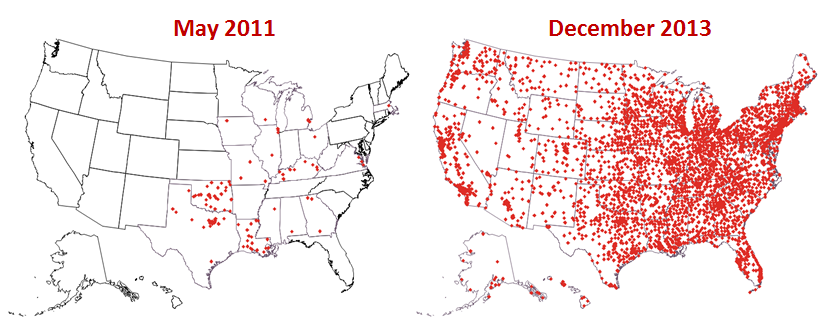
\includegraphics[scale=.6]{Objects/QS-Hospitals-Receiving-Payments-for-MU-and-Adoption.png}
    \caption*{Source: HealthIT.gov}
    \label{fig:meanuse}
\end{figure}

\import{Table Code}{overall stats.tex}

\import{Table Code}{split stats.tex}

\begin{figure}[p]
\centering
    \caption{Treatment Variables Over Time}
    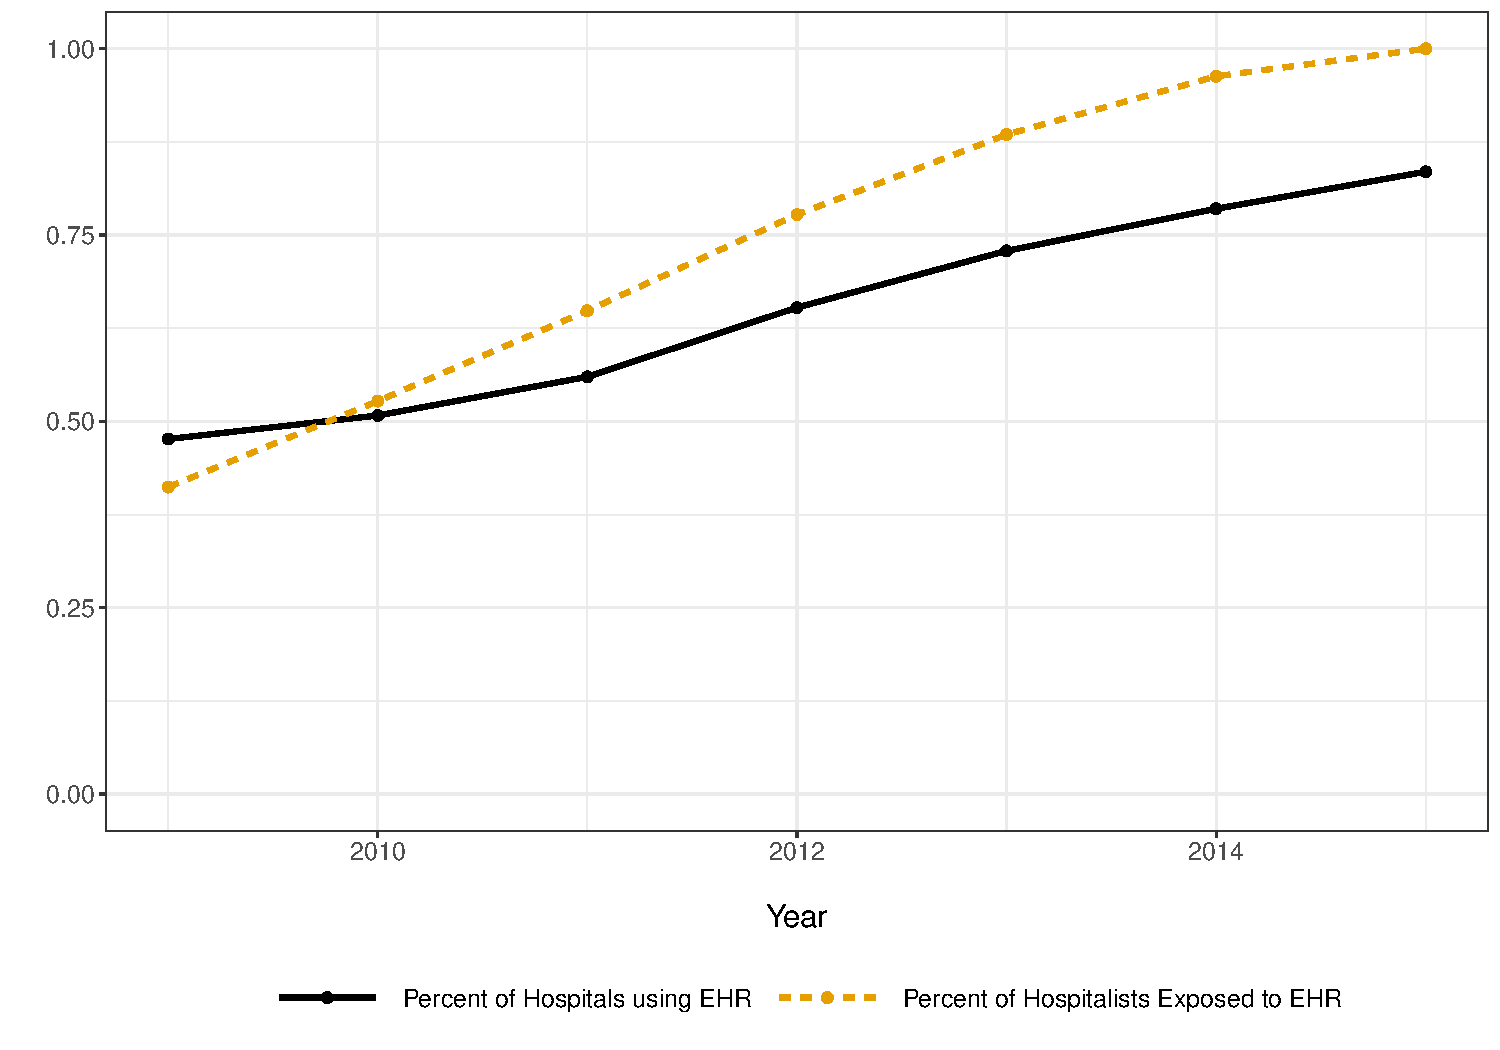
\includegraphics[scale=.55]{Objects/sum_stats_year.pdf}
    \label{fig:treatmentgraph}
\end{figure}

\begin{figure}[p]
    \centering
    \caption{Effect of EHR Exposure on Retirement}
    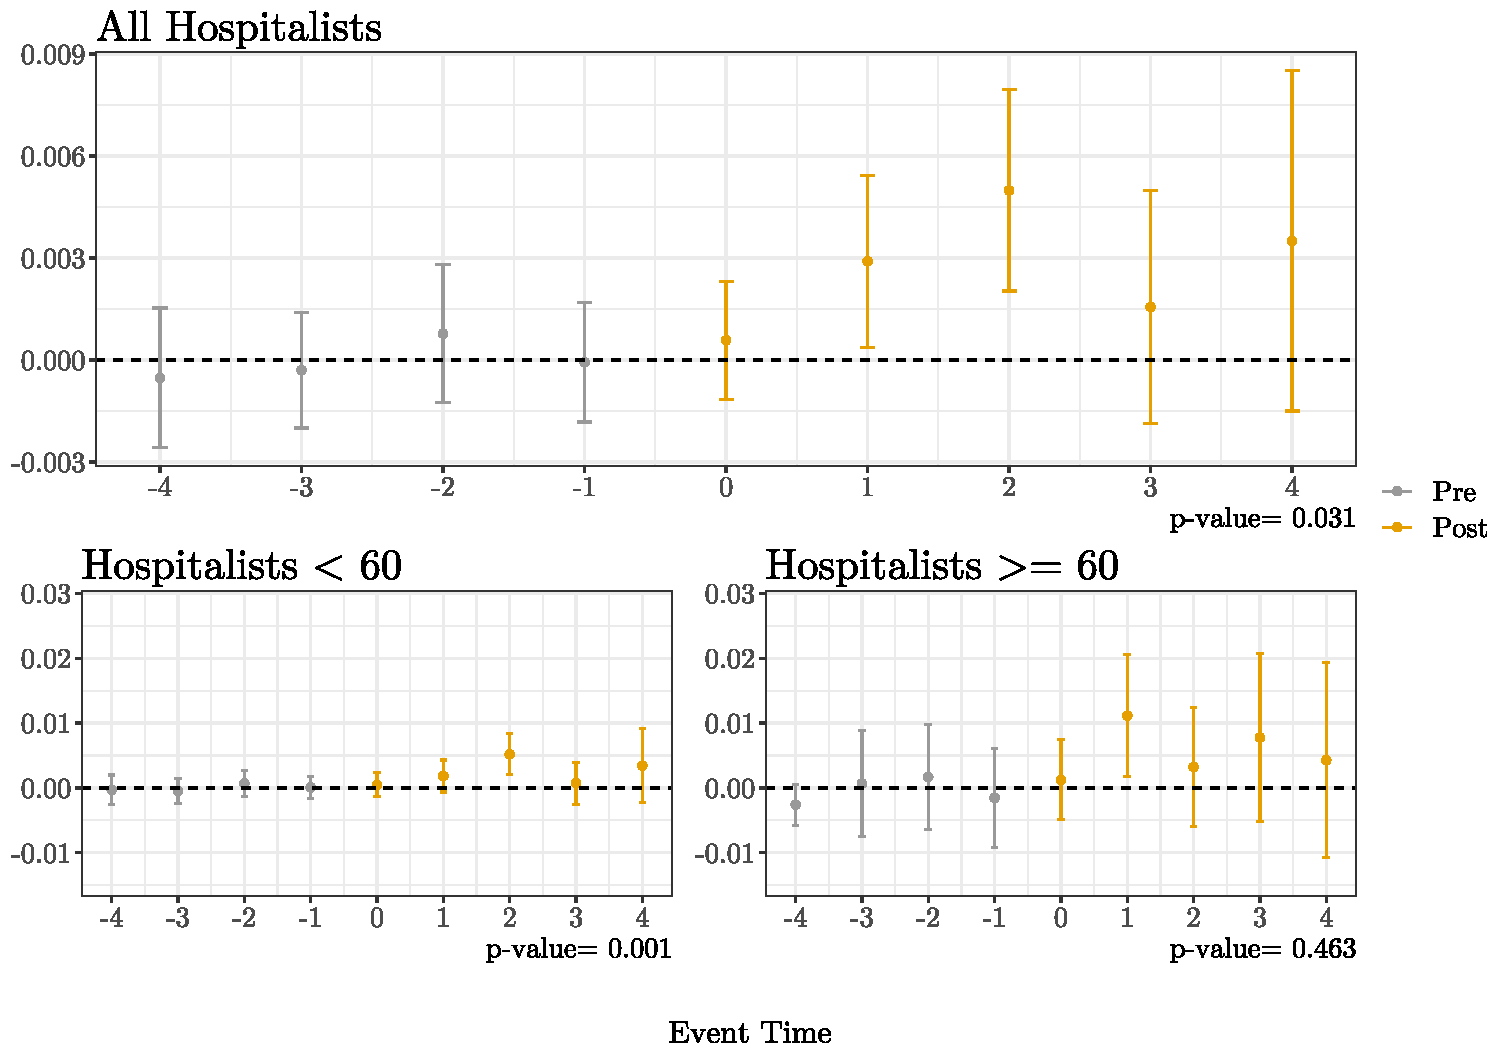
\includegraphics[scale=.57]{Objects/retire_plot.pdf}
    \label{fig:retirefirst}
\end{figure}

\begin{figure}[p]
    \centering
    \caption{Effect of EHR Exposure on Likelihood of Working in Office}
    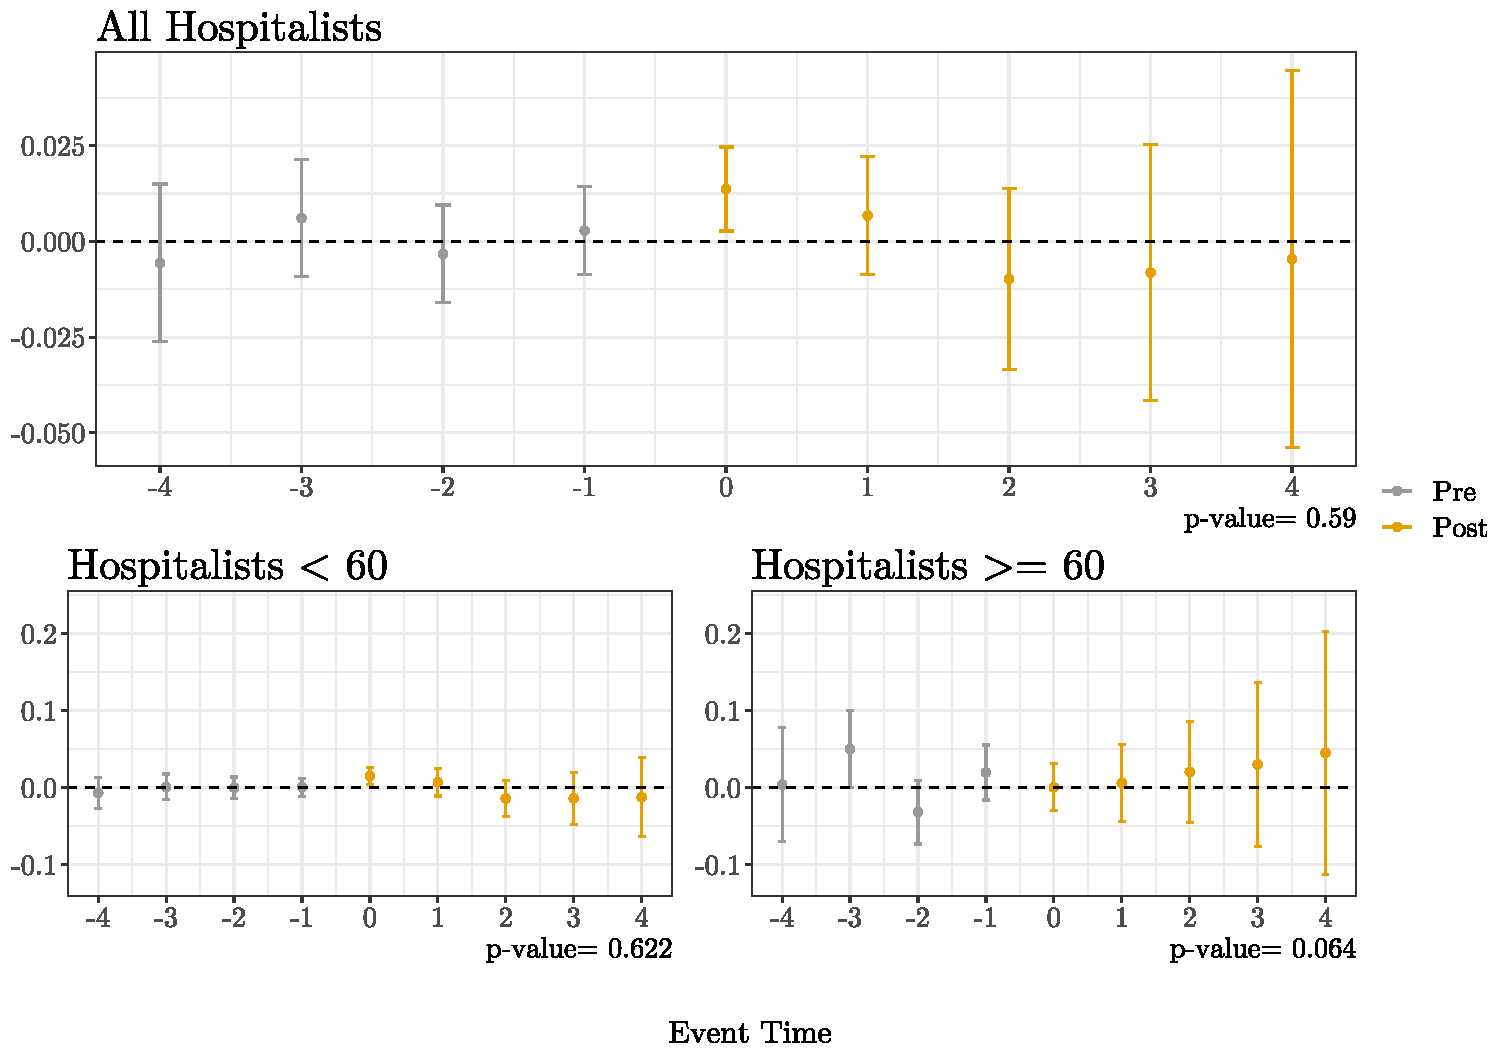
\includegraphics[scale=.57]{Objects/officeind_plot.pdf}
    \label{fig:officefirst}
\end{figure}

\begin{figure}[p]
    \centering
    \caption{Effect of EHR Exposure on Fraction of Total Patients Seen in Office}
    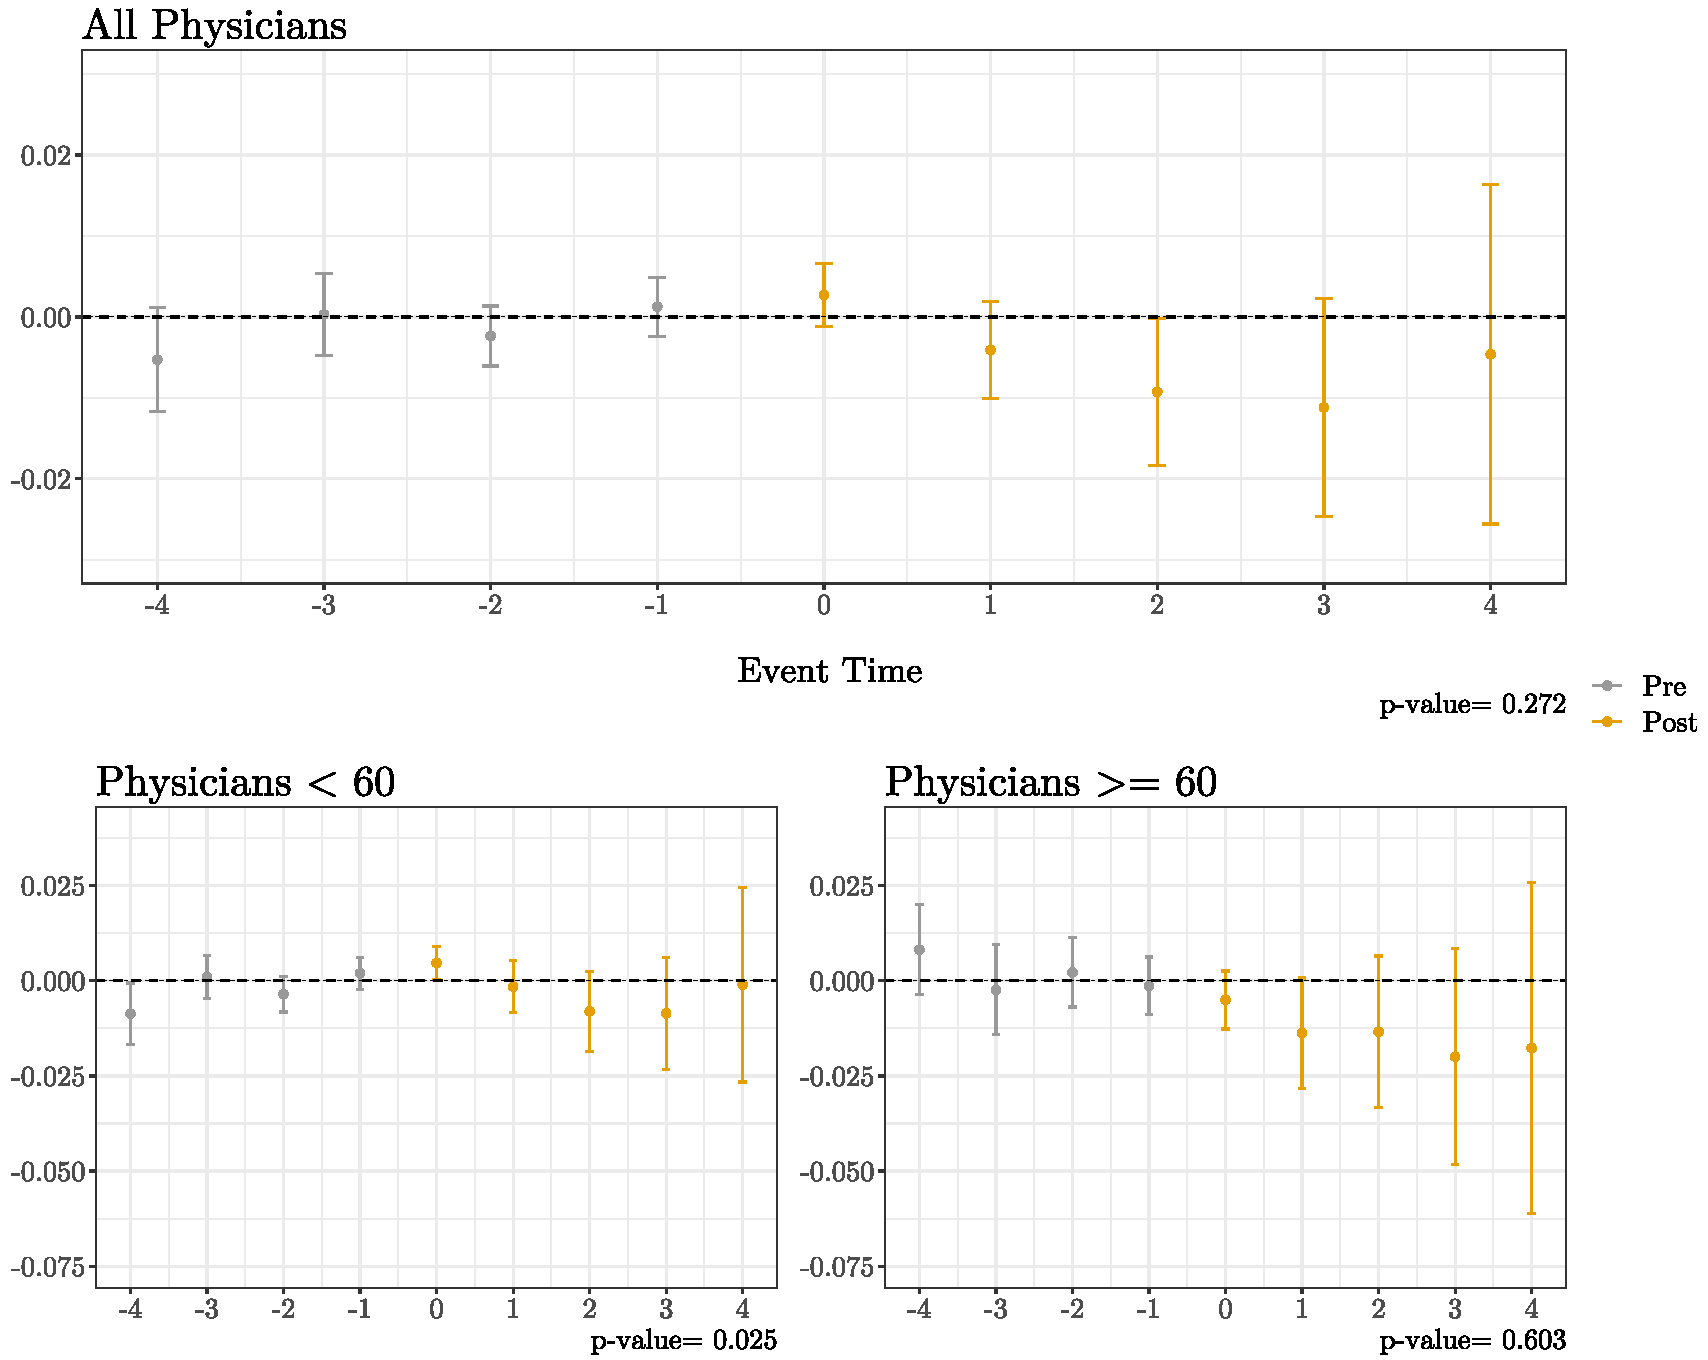
\includegraphics[scale=.57]{Objects/officefrac_plot.pdf}
    \label{fig:officesecond}
\end{figure}

\begin{figure}[p]
    \centering
    \caption{Effect of EHR Exposure on Likelihood of Changing Zip Codes}
    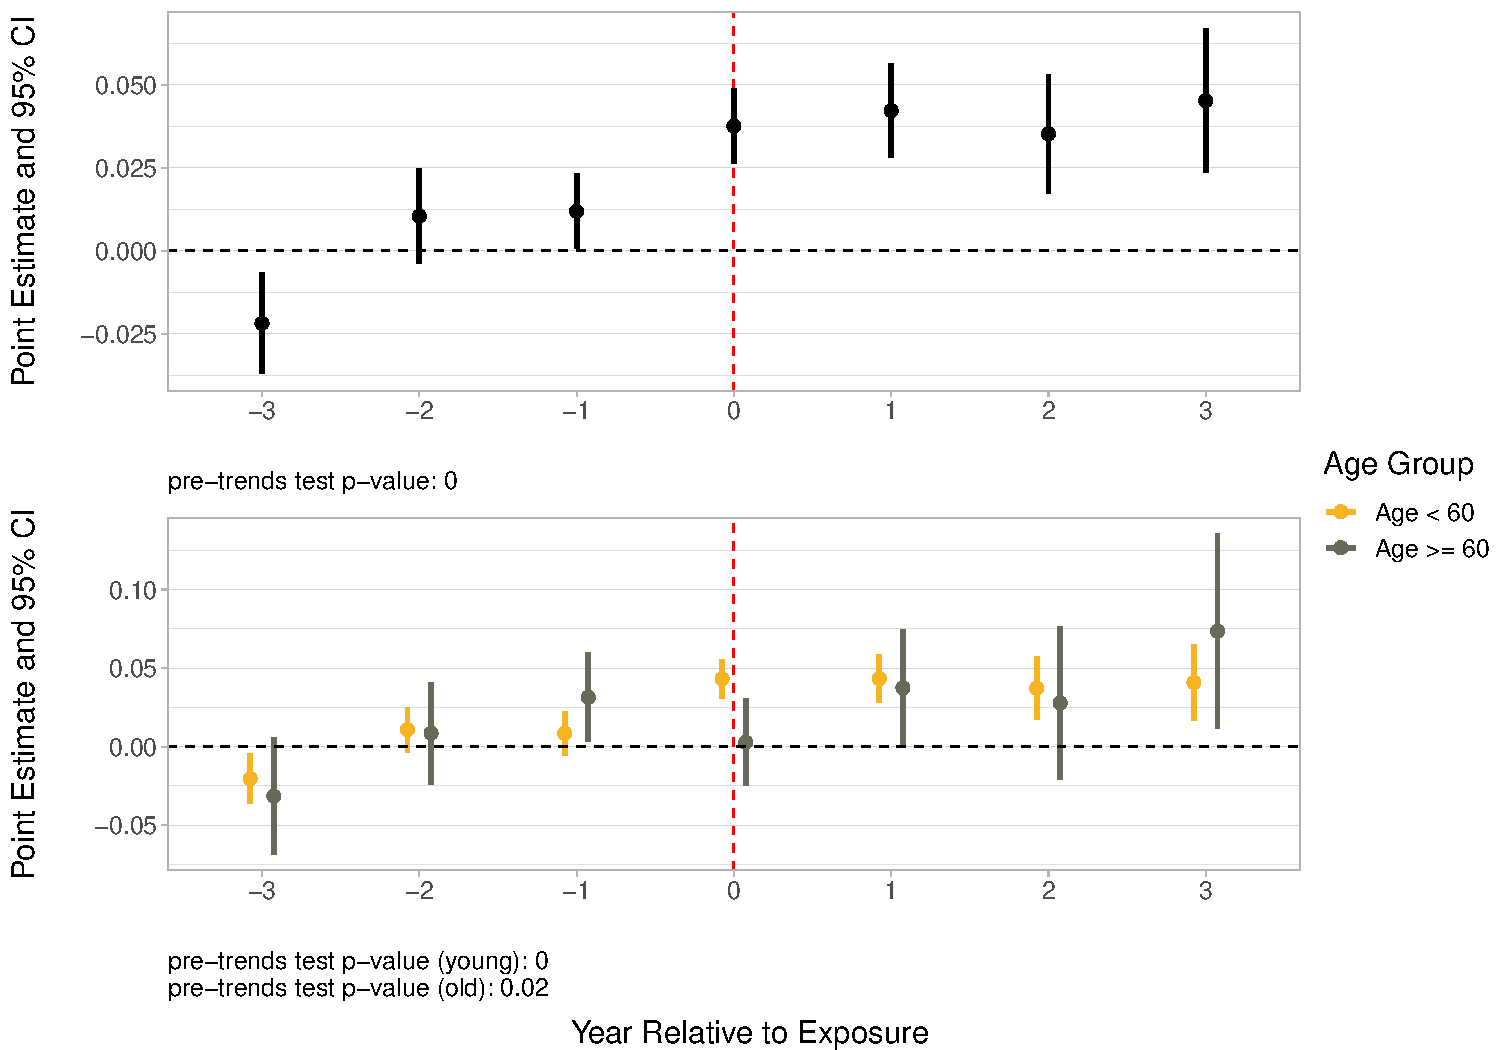
\includegraphics[scale=.57]{Objects/zip_plot.pdf}
    \label{fig:zip}
\end{figure}

\begin{figure}[p]
    \centering
    \caption{Effect of EHR Exposure on Patient Count}
    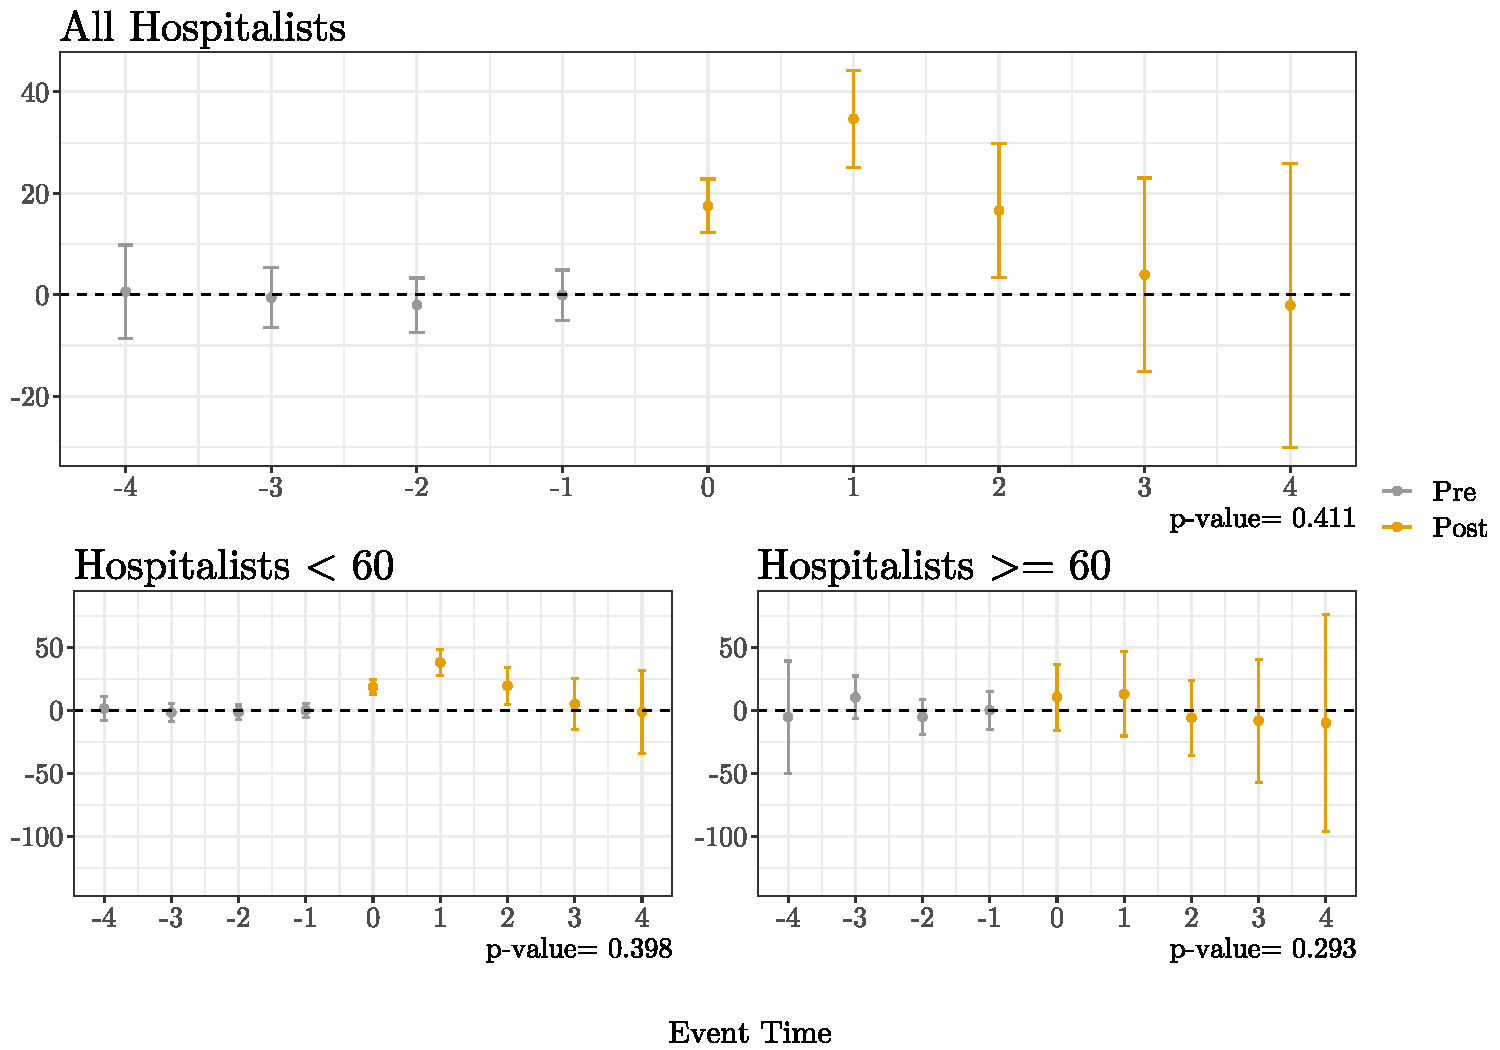
\includegraphics[scale=.57]{Objects/patient_plot.pdf}
    \label{fig:patient}
\end{figure}

\begin{figure}[p]
    \centering
    \caption{Effect of EHR Exposure on Claim Count}
    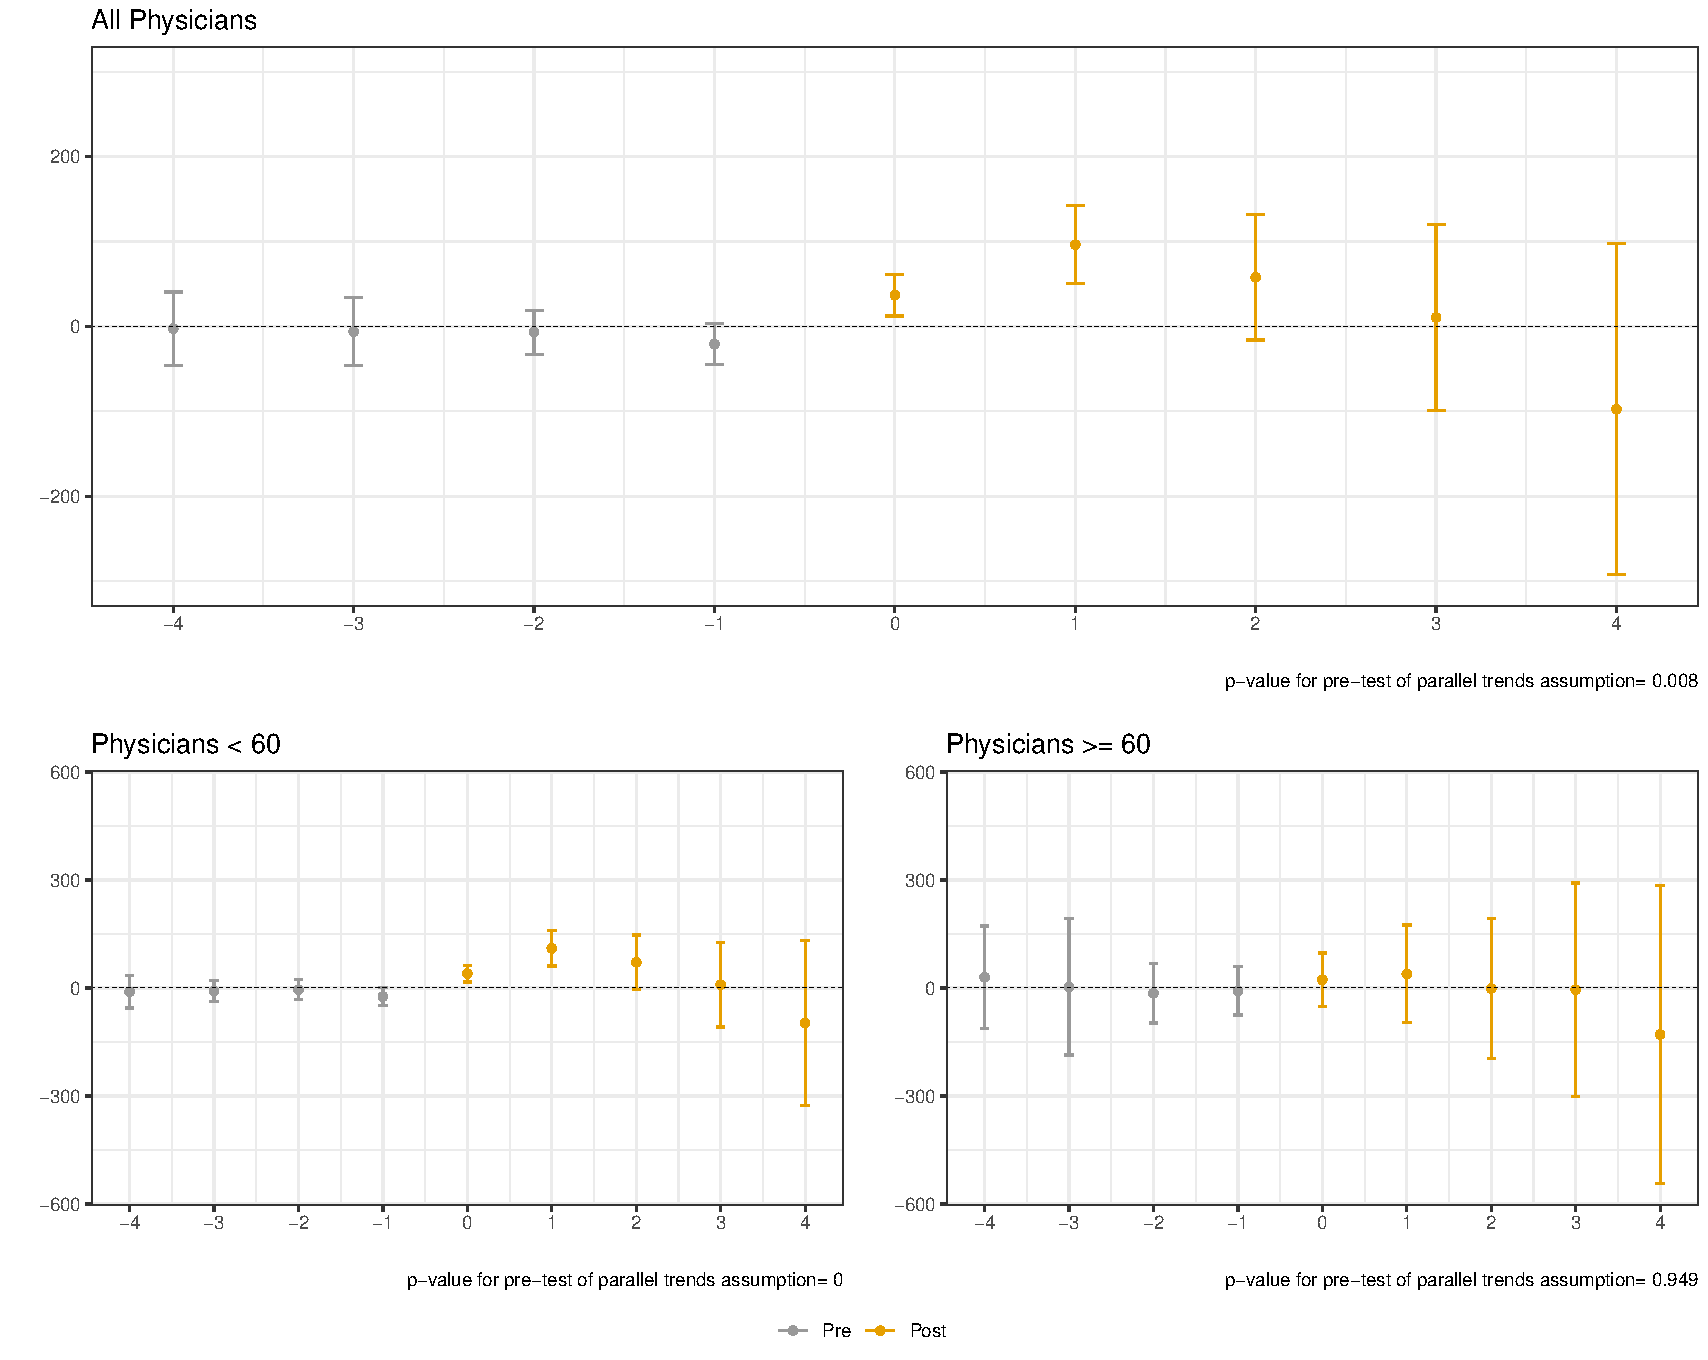
\includegraphics[scale=.57]{Objects/claim_plot.pdf}
    \label{fig:claim}
\end{figure}

\begin{figure}[p]
\centering
\caption{Frequency of Data Assistant Enumeration by Year}
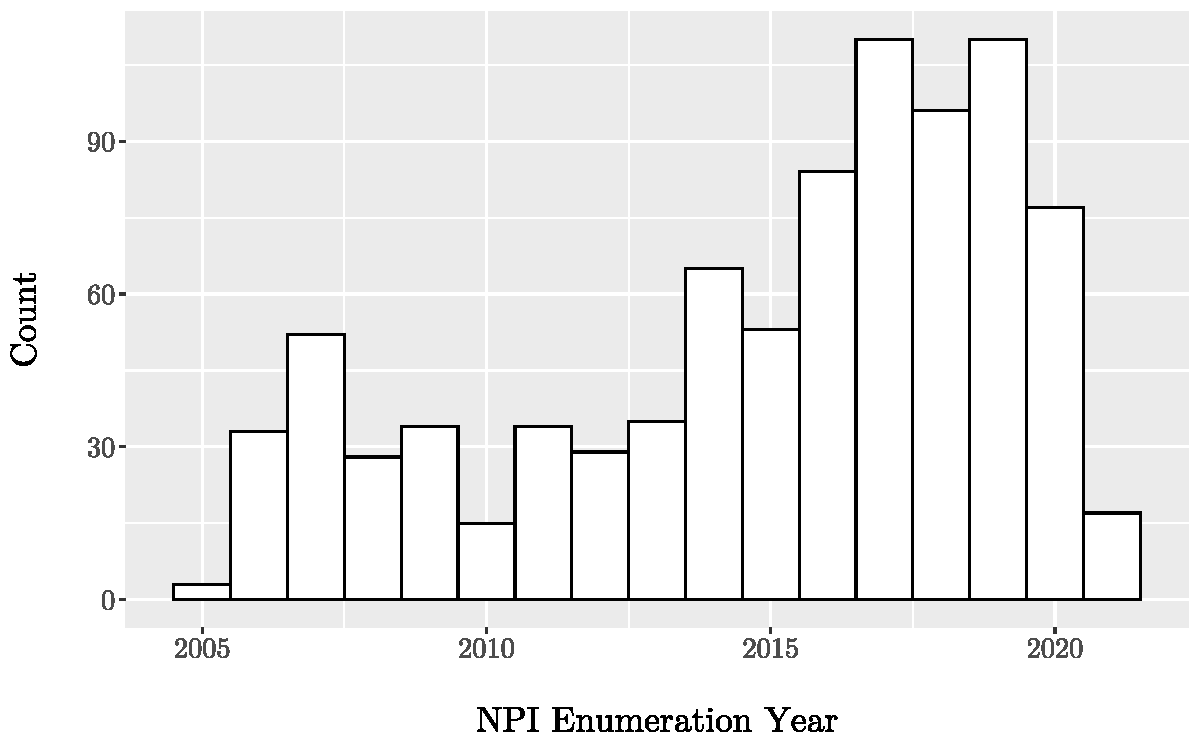
\includegraphics[scale=.5]{Objects/dataassistant_histogram.pdf}
\label{fig:dataassistant_histogram}
\end{figure}






\clearpage


\renewcommand*{\bibfont}{\footnotesize}

\printbibliography










\end{document}